\documentclass{article}

% if you need to pass options to natbib, use, e.g.:
%     \PassOptionsToPackage{numbers, compress}{natbib}
% before loading neurips_2018

% ready for submission
% \usepackage{neurips_2018}

% to compile a preprint version, e.g., for submission to arXiv, add add the
% [preprint] option:
%     \usepackage[preprint]{neurips_2018}

% to compile a camera-ready version, add the [final] option, e.g.:
     \usepackage[final]{nips_2018}

% to avoid loading the natbib package, add option nonatbib:
%     \usepackage[nonatbib]{neurips_2018}

\usepackage[utf8]{inputenc} % allow utf-8 input
\usepackage[T1]{fontenc}    % use 8-bit T1 fonts
\usepackage{hyperref}       % hyperlinks
\usepackage{url}            % simple URL typesetting
\usepackage{booktabs}       % professional-quality tables
\usepackage{amsfonts}       % blackboard math symbols
\usepackage{nicefrac}       % compact symbols for 1/2, etc.
\usepackage{microtype}      % microtypography
\usepackage{graphicx}
\usepackage{CJKutf8}
\usepackage{amsfonts,amssymb,amsmath}


\title{《人工神经网络》大作业终期报告}

% The \author macro works with any number of authors. There are two commands
% used to separate the names and addresses of multiple authors: \And and \AND.
%
% Using \And between authors leaves it to LaTeX to determine where to break the
% lines. Using \AND forces a line break at that point. So, if LaTeX puts 3 of 4
% authors names on the first line, and the last on the second line, try using
% \AND instead of \And before the third author name.

\author{%
  陶天骅 \\
  2017010255 \\
  计算机系 \\
  \texttt{tth17@mails.tsinghua.edu.cn} \\
  %% examples of more authors
  \And
  杨雅儒\\
  2017011071 \\
  计算机系 \\
  \texttt{yangyr17@mails.tinghua.edu.cn
  } \\
  %% \And
  %% Coauthor \\
  %% Affiliation \\
  %% Address \\
  %% \texttt{email} \\
}

\begin{document}
% \nipsfinalcopy is no longer used
\begin{CJK*}{UTF8}{gbsn}
\maketitle


\begin{abstract}

本课题尝试构建一个神经网络,用于自动生成尽可能真实的风景图片。我们分别对AutoEncoder、GAN、DCGAN、WGAN、StackGAN等诸多方案进行了尝试和对比,尽可能提高训练的稳定性,并最终在采用 DCGAN 的网络下得到了较好的结果。

\end{abstract}

\section{引言}

  我们一开始希望构建一个神经网络以及一些简单的界面,可以根据用户提供的一些特征的比例,自动生成一张尽可能真实且清晰的风景图片。首先在利用已有知识的情况下,我们尝试了使用 autoEncoder,但是即便是在经过多次调整尝试之后,效果仍然很不理想。在经过文献查阅之后,我们决定尝试使用生成对抗网络(Generative Adversarial Networks, GAN)[1] 来解决问题,并且为了提高清晰度使用了 stackGAN [4, 8, 9]对已生成的低清晰度图片进行再次对抗生成,以得到更高清的图片。接下来我们还参考了 Radford 等与 DCGAN 相关的工作[5],向网络中添加了卷积层,并进行了若干优化。

  尽管使用 DCGAN,加上一些训练技巧并且小心调参的情况下,已经能够得到不错的结果,但训练的稳定性问题一直没有得到解决。一方面,我们尝试了设计一个自适应的算法来自动调整训练过程,在尽可能小的影响训练质量的情况下,矫正训练中出现的过度不均衡的情况;另一方面,我们参考了 Arjovsky 等与 Wasserstein GAN (WGAN) 相关的工作 [11, 12],并且尝试使用其中的 Earth-Mover(EM) 距离,结合之前实现的 DCGAN 来解决问题。尽管这样有效提高了训练的稳定性,但由于 WGAN 在对每一层的网络参数调整上过于简单地使用 weight clipping,导致我们尝试用更深层的网络生成更高清的图片时出现了梯度消失的问题。

  最终,由于 WGAN 实际产生图片的效果同 DCGAN 差不多,而 DCGAN 在使用一定训练技巧的情况下已经能够比较稳定地产生较为优质且高清的图片,我们还是决定使用 DCGAN 作为了最终的网络方案,并且在各个数据集上进行了测试。另外对于我们一开始的目标——用户的比例选择以及界面等,在 GAN 的训练难度本身就很高的情况下已经没有足够的时间完成,但我们仍参阅了一些相关的文献 [2, 6],并大致有了一些解决方案。总之,虽然一开始的目标没有完成,但是我们确实已经向它迈进了一大步,并获得了足够的收获和成果。

\section{相关工作}

  自从 2014 年 Ian Goodfellow 等 [1] 设计出了起,各种各样的 GAN 变种便开始出现,研究者们在不断尝试提高 GAN 质量的同时,也尝试着将 GAN 应用于各种各样的场合。在应用方面,最常见的一种应用便是生成图像,除了本文中比较直接的生成图像方法以外,还有加入一些条件或风格的生成图像 [2, 6] 的 CGAN 和 StyleGAN 等,也可以用 CGAN 来做有监督的图像到图像的生成,而 [13, 14] 中的 CycleGAN 和 DualGAN 还能做到无监督的图像到图像生成,这些可以应用到风格转换等。另外还有例如 [4] 中做的文本到图像的生成等。

  而在质量提高方面,又可粗略地分为两部分,一是提高训练的稳定性,二是提高生成图像的质量。在稳定性提高上本文主要参考了 [11, 12],在 [11] 中 Arjovsky 等尝试了研究 GAN 训练不稳定的本质原因,即当 Discriminator 训练过优时将导致 Generator 的训练出现梯度消失。之后又在 [12] 中提出了 WGAN,使用 EM 距离替代原本的 JS 散度,使得在 Discriminator 训练得越好的情况下,Generator 训练的效果也越好。不过正如引言中所述的,WGAN 过于简单地使用 weight clipping 导致出现一些问题,于是 Gulrajani 等又提出了改进之后的 WGAN-GP [15],使用梯度惩罚来代替简单的 weight clipping,实现了更好的效果。在提高生成图像质量上,本文主要考虑到的是图片的清晰度,而 StackGAN [4, 8, 9] 的相关工作便利用分层的思想,逐步提高生成的图片尺寸,以达到生成高清图片的目的。当然还有一些更加强大的 GAN 模型,但由于受算力和时间等限制,本课题便没有对其深入研究。

\section{方法}

  \subsection{训练目标}
  
	 \subsubsection{DCGAN}

	 对于我们使用的 GAN、DCGAN 以及 StackGAN,用 D 表示判别器(discriminator),G 表示生成器(generator),训练目标如下:
	
	 \begin{equation}
	   \min_G\max_D V(D, G) = \mathbb{E}_{x\sim p_{data}(x)}[\log D(x)] + \mathbb{E}_{z\sim p_z(z)}[log(1-D(G(z)))].
	 \end{equation}
	 
	 于是考虑分别构建 D、G 两部分网络,并且进行轮流训练,在训练 D 和 G 时都分别需要固定另一方的网络。
    
    \subsubsection{WGAN}
   
    根据 [11] 的推导,式(1)在最优判别器 $D^*$ 下,实际上有:
    
    \begin{equation}
    \begin{aligned}
	  &\mathbb{E}_{x\sim p_{data}(x)}[\log D^*(x)] + \mathbb{E}_{z\sim p_z(z)}[log(1-D^*(G(z)))] \\
	  = &\mathbb{E}_{x\sim P_r}[\log D^*(x)] + \mathbb{E}_{x\sim P_g}[log(1-D^*(x))] \\
	  = &2JS(p_{data} || p_{gen}) - 2\log 2
	\end{aligned}
    \end{equation}

	而 Earth-Mover (EM) 距离定义如下:
	
	\begin{equation}
	  W(P_r, P_g) = \inf_{\gamma \sim \Pi(P_r, P_g)} \mathbb{E}_{(x, y) \sim \gamma}[||x-y||]
	\end{equation}
	
	使用 EM 距离而不是 JS 散度的优点即,即便两个分布没有重叠,EM 距离仍然能够反映它们的远近关系,而 JS 散度并不能做到这一点。再利用 [12] 的思路和数学推导,我们便可以得到 WGAN 具体的网络形式。
	
  \subsection{DCGAN 模型}
  
	整体分为两部分,Generator 部分和 Discriminator 部分,可以参考 Figure 1, 2,参数和尺寸在图中标注。
	
	\begin{figure}[htbp]
		\begin{minipage}{0.5\linewidth}
			\centering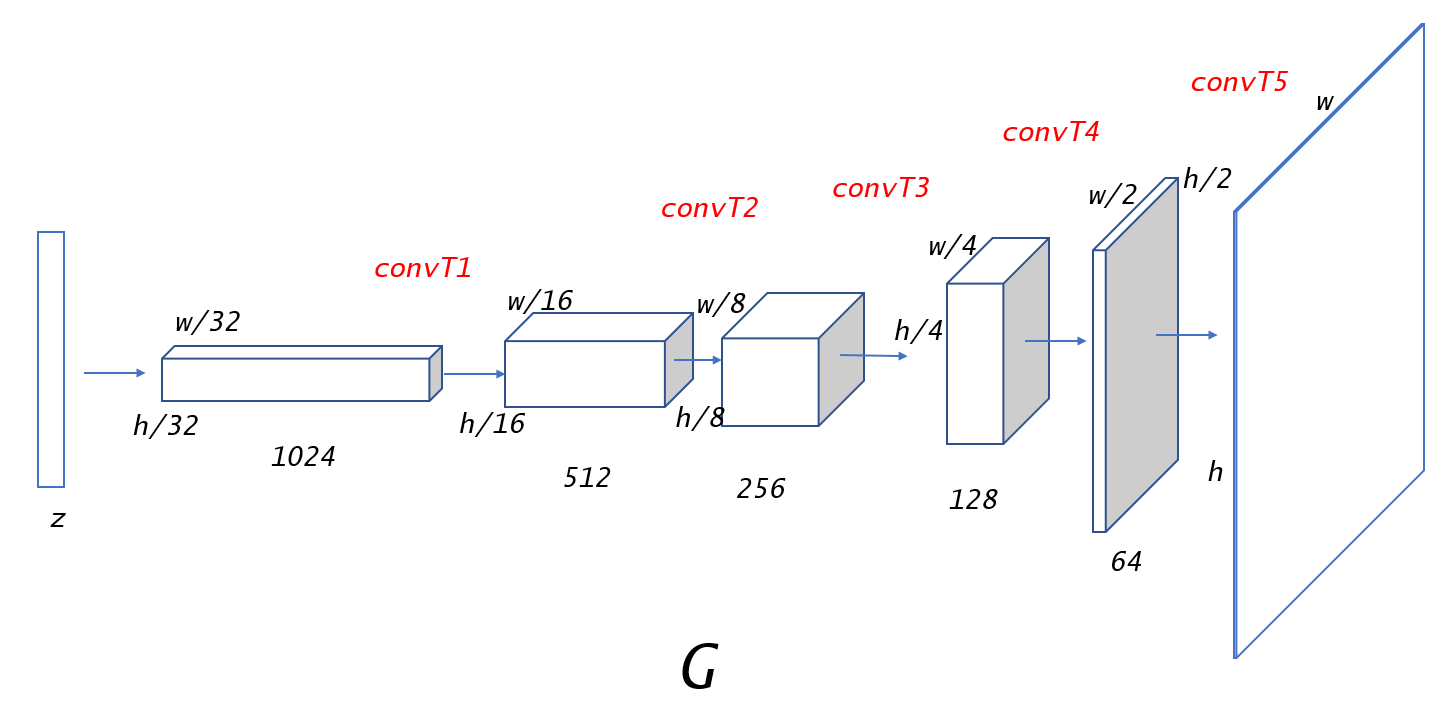
\includegraphics[scale=0.13]{res/DCGAN_generator.png}
			\caption{The model of generator in DCGAN.}
		\end{minipage}
		\begin{minipage}{0.5\linewidth}
			\centering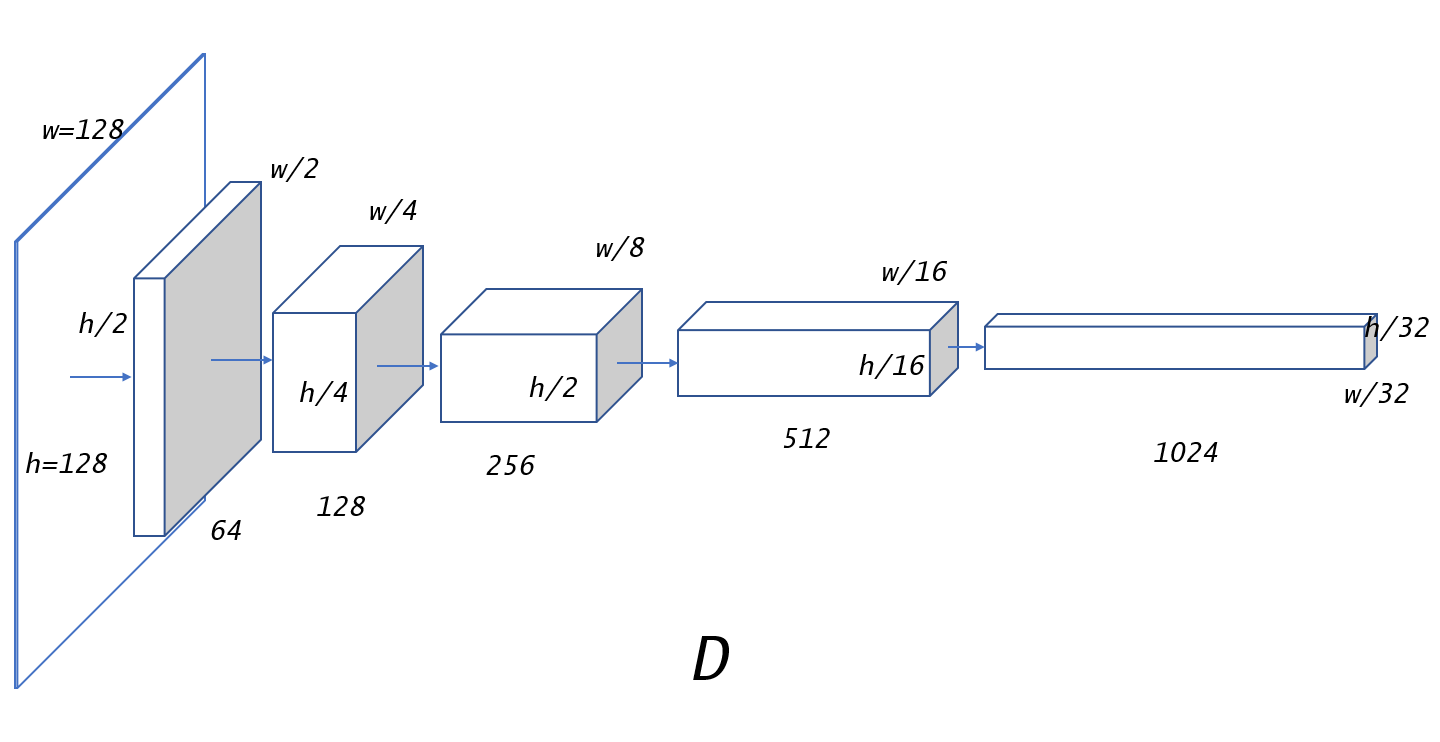
\includegraphics[scale=0.13]{res/DCGAN_discriminator.png}
			\caption{The model of discriminator in DCGAN.}
		\end{minipage}
	\end{figure}
	
	在 Generator 中,除了最后一层以 tanh 作为激活函数以外,其它层均以 relu 作为激活函数;在 Discriminator 中,除了最后一层以 sigmoid 作为激活函数以外,其它层均以 leakyRelu 作为激活函数。最终的 loss 采用交叉熵误差函数。
	
  
  \subsection{WGAN 模型}

	在 DCGAN 模型的基础上,为每一层的参数增加了 clipping,并且删去了 Discriminator 最后的激活函数。另外在每一个conv/deconv层之后加入了 BatchNormalization,并在 Discriminator 的每一个卷积层激活之后加入了 Dropout 层。

	\begin{figure}[htbp]
		\begin{minipage}{0.5\linewidth}
			\centering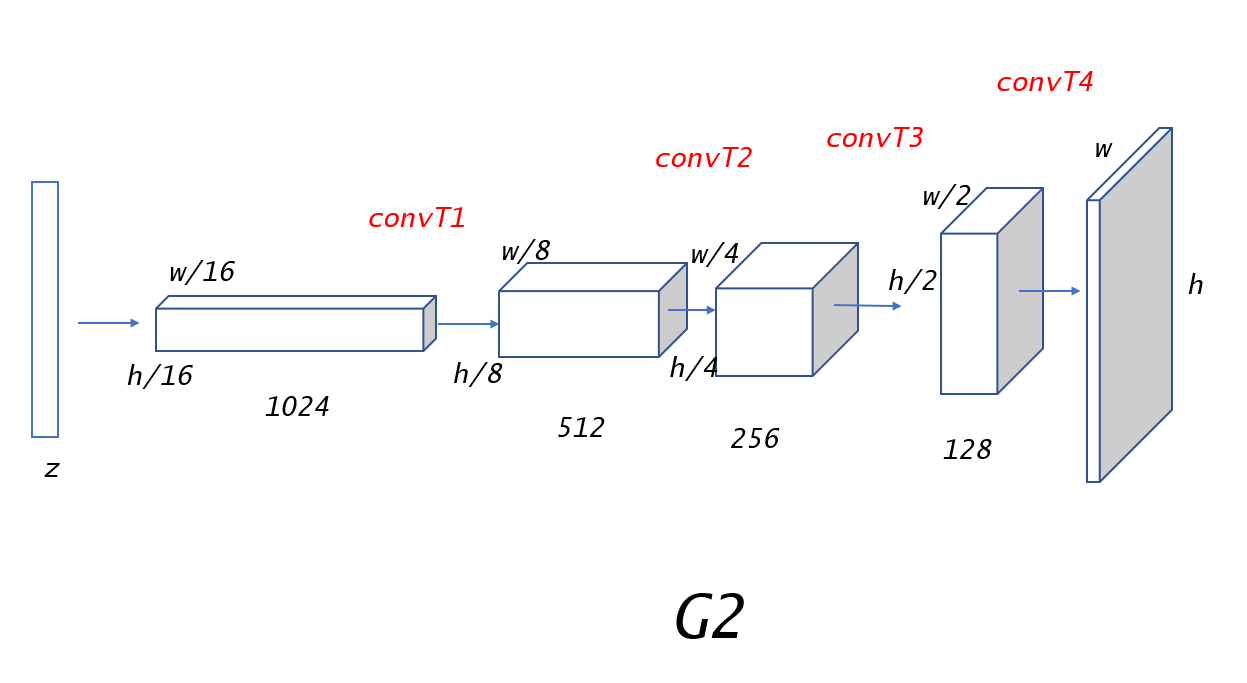
\includegraphics[scale=0.13]{res/WGAN_generator.png}
			\caption{The model of generator in WGAN.}
		\end{minipage}
		\begin{minipage}{0.5\linewidth}
			\centering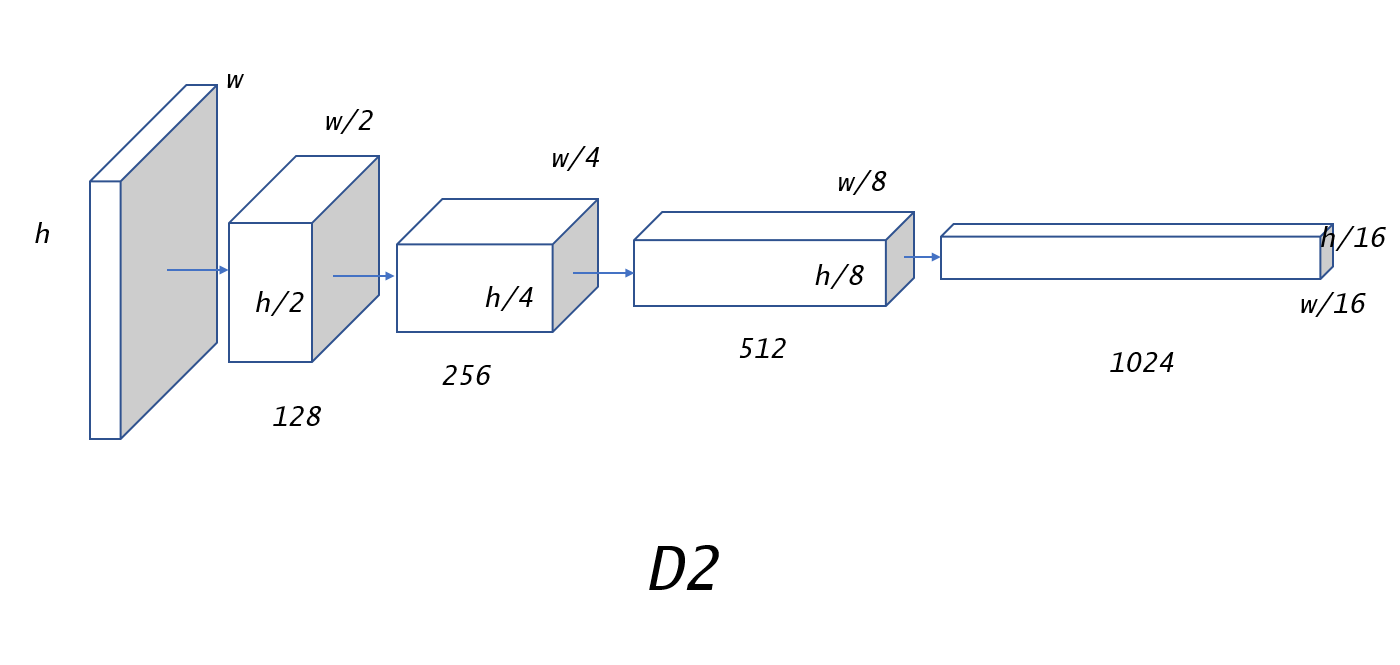
\includegraphics[scale=0.13]{res/WGAN_discriminator.png}
			\caption{The model of discriminator in WGAN.}
		\end{minipage}
	\end{figure}
  
	并且使用如下 loss,将其称为 Wasserstein Loss:
	
	\begin{equation}
		loss = \frac{1}{L} \Sigma_{i=1}^L y_{label} * y_{pred} 
	\end{equation}
	
	其中 $y_{label}$ 表示实际是否为真实图片,$y_{pred}$ 表示 Discriminator 的输出结果。

\section{实验}

  由于最终我们的 WGAN 并没有在尺寸更大的图片中取得很好的结果,在本课题中仅作为一个稳定性优化方向给出,更具有理论意义。所以为了减少冗余,在实验部分就省去了 WGAN 相关的实验信息,而仅以在大尺寸图片中表现仍旧较好的 DCGAN 作为最终网络,给出具体实验信息。

  \subsection{数据集}
	我们使用了六组数据集,详细见下表格,并且对于每一组数据集进行了resize,分为 64*64, 128*128, 256*256,分别进行训练。数据大多由我们自行爬取和整理,可以在如下链接中下载: cloud.tsinghua.edu.cn/d/c00d7f1e66914948937e/。
	
	\begin{table}[htbp]
		\begin{center}
			\begin{tabular}{|c|c|c|c|c|c|c|}
				\hline
				Name	  & landscape	& mountains	& birds & lake  & dog   & cat \\
				\hline
				Pictures  &	61132		& 14090     & 11788 & 13840 & 12462 & 12467   \\
				\hline
			\end{tabular}
			\vspace{10pt}
			\caption{The name and number of pictures of the datasets.}
		\end{center}
	\end{table}

	这里展示出部分数据集的一些例子。
	
	\begin{figure}[htbp]
		\begin{minipage}{0.5\linewidth}
			\centering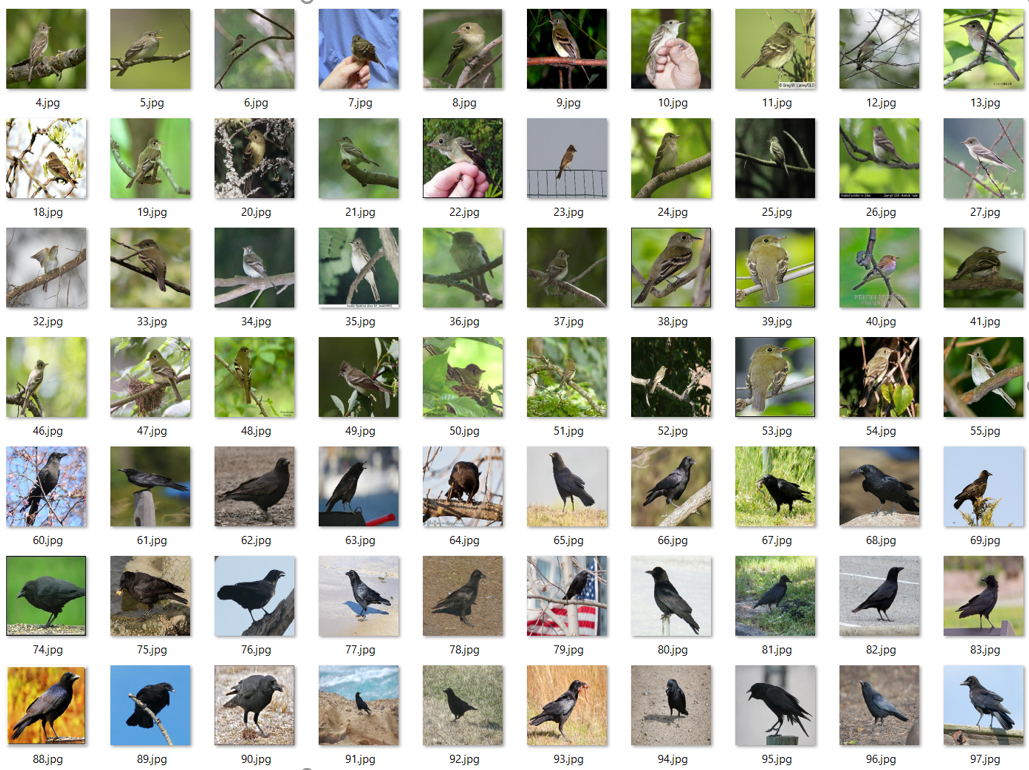
\includegraphics[scale=0.15]{res/bird.png}
			\caption{Some pictures in bird datasets}
		\end{minipage}
		\begin{minipage}{0.5\linewidth}
			\centering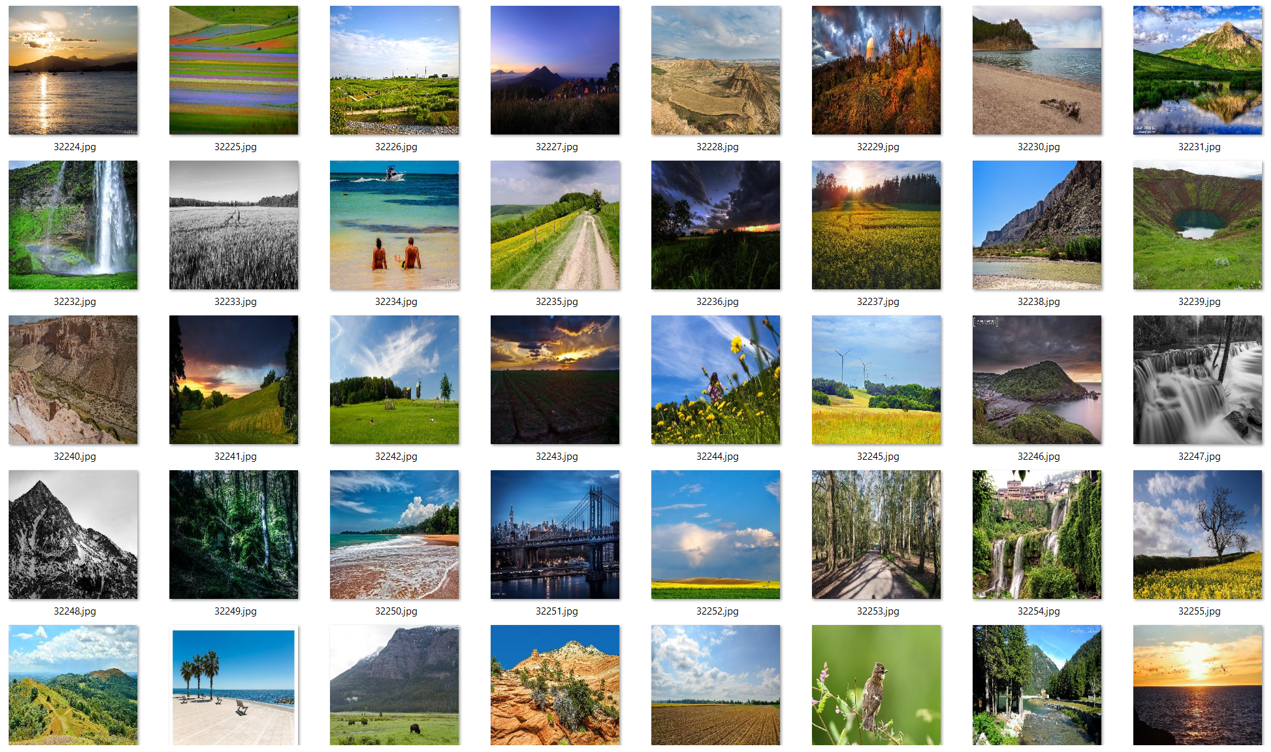
\includegraphics[scale=0.15]{res/landscape.png}
			\caption{Some pictures in landscape datasets}
		\end{minipage}
	\end{figure}
	
	
  \subsection{参数设置}
    

  \subsection{baseline模型}

	我们以文献        

  \subsection{实验结果与分析}

	
  [TODO: 注意需要提供量化数值分析]

\section{结论}

在本次课题中,经过对不同模型在生成图片上的研究,以及对参数的不断调整和试验,我们发现在较为朴素的 DCGAN 上加上一些训练技巧便已经可以达到较好的水准。

[TODO:这部分需要指标结果]

  在分工上,陶天骅同学在整体上对本次课题进行了方向规划和指导,收集了山、鸟、猫、狗、森林、湖等数据集并进行图片的 resize 处理,并对 AutoEncoder、朴素GAN、DCGAN、StackGAN 等分别进行了尝试,并加入了 Inception Score 对最终网络进行评价 [TODO: 有无工作补充?]。杨雅儒同学收集了 Kaggle 上的风景数据集,并独立进行了对 DCGAN 的搭建和调参,设计了一个自适应算法,并尝试对其改进来稳定 DCGAN 的训练,在参阅文献发现不稳定的本质原因之后,进行了一定的推导验证并尝试更换训练目标以使用 WGAN 来进行训练。文档方面,陶天骅同学撰写了中期报告和展示PPT的大部分内容,杨雅儒同学撰写了结题报告的大部分内容。

\section*{参考文献}

\small

[1] Ian J. Goodfellow, Jean Pouget-Abadie, Mehdi Mirza , et al. Generative Adversarial Networks[J]. 2014.

[2] Karras, Tero, Laine, Samuli, Aila, Timo. A Style-Based Generator Architecture for Generative Adversarial Networks[J]. 2019

[3] M. Heusel, H. Ramsauer, T. Unterthiner, B. Nessler, and S. Hochreiter. GANs trained by a two time-scale update rule converge to a local Nash equilibrium. In Proc. NIPS, pages 6626–6637, 2017.

[4] Zhang H , Xu T , Li H , et al. StackGAN: Text to Photo-realistic Image Synthesis with Stacked Generative Adversarial Networks[J]. 2016.

[5] A. Radford, L. Metz, S. Chintala. Unsupervised Representation Learning with Deep Convolutional Generative Adversarial Networks[J]. 2016.

[6] M. Mirza, S. Osindero. Conditional Generative Adversarial Nets[J]. 2014.

[7] Heusel M , Ramsauer H , Unterthiner T , et al. GANs Trained by a Two Time-Scale Update Rule Converge to a Local Nash Equilibrium[J]. 2017.

[8] Zhang H , Xu T , Li H , et al. StackGAN: Text to Photo-realistic Image Synthesis with Stacked Generative Adversarial Networks[J]. 2016.

[9] Han Z , Tao X , Hongsheng L , et al. StackGAN++: Realistic Image Synthesis with Stacked Generative Adversarial Networks[J]. IEEE Transactions on Pattern Analysis and Machine Intelligence, 2018:1-1.

[10] Diederik P Kingma, Max Welling. Auto-Encoding Variational Bayes[J]. 2014

[11] Arjovsky M , Bottou, L\'{e}on. Towards Principled Methods for Training Generative Adversarial Networks[J]. Stat, 2017.

[12] Martin Arjovsky, Soumith Chintala, L\'{e}on Bottou. Wasserstein GAN[J]. 2017.

[13] Jun-Yan Zhu, Taesung Park, Phillip Isola, Alexei A. Efros. Unpaired Image-to-Image Translation using Cycle-Consistent Adversarial Networks[J]. 2018.

[14] Yi Z, Zhang H, Tan P , et al. DualGAN: Unsupervised Dual Learning for Image-to-Image Translation[J]. 2018

[15] I. Gulrajani, F. Ahmed, M. Arjovsky , et at. Improved Training of Wasserstein GANs[J]. 2017

\end{CJK*}
\end{document}
